% \PassOptionsToClass{negatif}{m53beamer}
% \PassOptionsToClass{withsidebar}{m53beamer}
% \PassOptionsToClass{handout}{m53beamer}
\documentclass{m53beamer}

% ---------------
\title{M53 - Partie 2}
%\author{Kroum Tzanev}
\date{octobre 2017}
% ---------------

\begin{document}

% ------- Le titre --------
\begin{frame}
  \titlepage
\end{frame}

% =======================================
\section{Rappels : espace euclidien}
% =======================================
% ~~~~~~~~~~~~~~~~~~~~~~~~~~~~~~~~~~~~~~~
\subsection{Définition}
% ~~~~~~~~~~~~~~~~~~~~~~~~~~~~~~~~~~~~~~~
% -----------
\begin{frame}{Rappels : définition espace vectoriel euclidien}
  Un espace vectoriel réel $\ev{E}$ de dimension finie est dit \alert{euclidien} s'il est muni d'une forme bilinéaire
    \begin{gather*}
      \ev{E} \times \ev{E} \longrightarrow \mathbb{R}\\
      (\vv{v},\vv{w}) \mapsto \scalprod{\vv{v}}{\vv{w}}
    \end{gather*}\vspace*{-1.4\baselineskip}
    \begin{itemize}[<+(1)->]
      \item symétrique : $\scalprod{\vv{v}}{\vv{w}} = \scalprod{\vv{w}}{\vv{v}}$,
      \item définie : $\scalprod{\vv{v}}{\vv{v}} = 0$ $\Leftrightarrow$ $\vv{v} = 0$,
      \item positive : $\scalprod{\vv{v}}{\vv{v}} \geq 0$.
    \end{itemize}\pause
  La structure euclidienne standard sur $\mathbb{R}^{n}$ est définie par
  \vspace*{-.7\baselineskip}
  \[
    \scalprod{(x_{1},\ldots,x_{n})}{(y_{1},\ldots,y_{n})}=x_{1}y_{1}+\cdots+x_{n}y_{n}.
  \]\pause
  Tout espace euclidien est isomorphe à $\mathbb{R}^{n}$ (avec sa structure standard),\pause
  via le choix (non canonique) d'une b.o.n.
\end{frame}

% ~~~~~~~~~~~~~~~~~~~~~~~~~~~~~~~~~~~~~~~
\subsection{Norme}
% ~~~~~~~~~~~~~~~~~~~~~~~~~~~~~~~~~~~~~~~
% -----------
\begin{frame}{Rappels : norme euclidienne}
  \begin{enumerate}[<+(1)->]
    \item La \alert{norme euclidienne} de cet espace est : $\norm{\vv{v}} = \sqrt{\scalprod{\vv{v}}{\vv{v}}}$.
    \item Et une formule inverse \myemph{(de polarisation)} est :
      \[
        \scalprod{\vv{v}}{\vv{w}} = \frac12\big( \norm{\vv{v}+\vv{w}}^{2} - \norm{\vv{v}}^{2} - \norm{\vv{w}}^{2}\big).
      \]
    \item De plus la norme et la produit scalaire sont reliés par \myemph{l'inégalité de Cauchy-Schwarz}
      \[
        \big|\scalprod{\vv{v}}{\vv{w}}\big| \leq \norm{\vv{v}}\norm{\vv{w}}.
      \]
    \item On dit que \alert{l'angle} entre $\vv{v}$ et $\vv{w}$ est $\alpha \in[0,\pi]$ si
      \[
        \scalprod{\vv{v}}{\vv{w}} = \cos(\alpha)\norm{\vv{v}}\norm{\vv{w}}.
      \]
  \end{enumerate}
\end{frame}

% ~~~~~~~~~~~~~~~~~~~~~~~~~~~~~~~~~~~~~~~
\subsection{Notations}
% ~~~~~~~~~~~~~~~~~~~~~~~~~~~~~~~~~~~~~~~
% -----------
\begin{frame}{Rappels : notations}
  \begin{enumerate}[<+(1)->]
    \item $\vv{v}\perp\vv{w} \Leftrightarrow \scalprod{\vv{v}}{\vv{w}}=0$.
    \item Soit $\ev{F}\subset\ev{E}$, alors $\ev{F}^{\perp}=\big\{\vv{v} \in \ev{E} \big|\ \forall \vv{w} \in \ev{F}, \vv{v}\perp\vv{w} \big\}$.
    \item Soit $\ev{F}_{1},\ev{F}_{2}\subset\ev{E}$, alors $\ev{F}_{1}\perp\ev{F}_{2} \Leftrightarrow \ev{F}_{1}\subset\ev{F}_{2}^{\perp}$.
    \item $\ev{E}$ est la somme directe orthogonale de deux sous-espaces vectoriels $\ev{F}_{1}$ et $\ev{F}_{2}$, noté $\ev{E}=\ev{F}_{1}\poplus\ev{F}_{2}$, \pause si $\ev{E}=\ev{F}_{1}\oplus\ev{F}_{2}$ et $\ev{F}_{1}\perp\ev{F}_{2}$.\pause\\
    Nous avons : $\ev{E}=\ev{F}_{1}\poplus\ev{F}_{2}$ $\Leftrightarrow$ $\ev{F}_{1}^{\perp} = \ev{F}_{2}$\pause $\Leftrightarrow$ $\ev{F}_{2}^{\perp} = \ev{F}_{1}$.
  \end{enumerate}
\end{frame}

% =======================================
\section{Espaces affines euclidiens}
% =======================================

% ~~~~~~~~~~~~~~~~~~~~~~~~~~~~~~~~~~~~~~~
\subsection{Définition}
% ~~~~~~~~~~~~~~~~~~~~~~~~~~~~~~~~~~~~~~~
% -----------
\begin{frame}{Définition d'un espace affine euclidien}
  \begin{definition}
    Un ensemble $\ens{E}$ est \alert{métrique} s'il est muni d'un application \alert{distance}\forsimple{\vspace*{-.7\baselineskip}}
    \begin{gather*}
      \ens{E} \times \ens{E} \longrightarrow \mathbb{R}_{+}\\
      (M,N) \mapsto d(M,N)
    \end{gather*}\vspace*{-.7\baselineskip}
    \begin{itemize}[<+(1)->]
      \item symétrique : $d(M,N) = d(N,M)$,
      \item séparée : $d(M,N) = 0$ $\Leftrightarrow$ $M=N$,
      \item inégalité triangulaire : $d(M,N)+d(N,P)\geq d(M,P)$.
    \end{itemize}
  \end{definition}\pause
  \begin{definition}
    Un espace affine $\ens{E}$ est dit \alert{euclidien} si son espace vectoriel de directions $\ev{E}$ est muni d'une structure euclidienne.\pause\\
    Et dans ce cas on pose la distance entre deux points
    \[
      d(A,B) = \norm{\vv{AB}}.
    \]
  \end{definition}
\end{frame}

% ~~~~~~~~~~~~~~~~~~~~~~~~~~~~~~~~~~~~~~~
\subsection{Distance entre parties}
% ~~~~~~~~~~~~~~~~~~~~~~~~~~~~~~~~~~~~~~~
% -----------
\begin{frame}{Distance entre parties}
  \begin{definition}
    Soit $\ens{A}$ et $\ens{B}$ deux parties d'un espace affine euclidien $\ens{E}$.
    On pose\forsimple{\vspace*{-.7\baselineskip}}
    \[
      d(\ens{A},\ens{B}) = \inf_{(M,N) \in \ens{A}\times\ens{B}}d(M,N).
    \]\forsimple{\vspace*{-.7\baselineskip}}
  \end{definition}
  \begin{enumerate}[<+(1)->]
    \item Si $\ens{A}$ est compacte et $\ens{B}$ est fermée, les deux non vides, alors il existe un couple de points $(M,N) \in \ens{A}\times\ens{B}$ tel que $d(\ens{A},\ens{B}) = d(M,N)$.\pause\\ Et pour $\ens{A}$ seulement fermée ?
    \item La propriété précédente reste vraie pour $\ens{A}$ et $\ens{B}$ des sous-espaces affines. De plus $\vv{MN}\perp(\vv{A}+\vv{B})$.
    \item Deux hyperplans distincts $\ens{F}$ et $\ens{G}$ de $\ens{E}$ sont parallèles ssi $d(\ens{F},\ens{G}) > 0$. \pause Et pour s.e.a. quelconques ?
    \item Deux sous-espaces affines $\ens{F}$ et $\ens{G}$ de $\ens{E}$ sont parallèles ssi $\forall (M,N) \in \ens{F}\times\ens{G}, d(M,\ens{G})=d(\ens{F},\ens{G})=d(\ens{F},N)$.
  \end{enumerate}
\end{frame}


% =======================================
\section{Isométries vectorielles}
% =======================================

% ~~~~~~~~~~~~~~~~~~~~~~~~~~~~~~~~~~~~~~~
\subsection{Définition}
% ~~~~~~~~~~~~~~~~~~~~~~~~~~~~~~~~~~~~~~~
% -----------
\begin{frame}{Rappels : isométrie vectorielle }
  \begin{defprop}
    L'application linéaire $\vv{\phi}$ est une \alert{isométrie} (dit également \alert{orthogonale}) de $\ev{E}$ si elle satisfait une des conditions équivalentes
    \begin{enumerate}[<+(1)->]
      \item $\forall \vv{v} \in \ev{E}$,
        \[
           \norm{\vv{\phi}(\vv{v})}=\norm{\vv{v}}.
        \]
      \item $\forall \vv{v},\vv{w} \in \ev{E}$,
        \[
          \scalprod{\vv{\phi}(\vv{v})}{\vv{\phi}(\vv{w})}=\scalprod{\vv{v}}{\vv{w}}.
        \]
      \item
        \[
          \vv{\phi}\circ\vv{\phi}^{t} = \id \pause\quad\Leftrightarrow\quad
          \vv{\phi}^{t}\circ\vv{\phi} = \id \pause\quad\Leftrightarrow\quad
          \vv{\phi}^{-1} = \vv{\phi}^{t}
        \]\forsimple{\vspace*{-.7\baselineskip}}
    \end{enumerate}
  \end{defprop}
\end{frame}

% -----------
\begin{frame}{Rappels : décomposition et spectre des isométries }
  \begin{enumerate}[<+(1)->]
    \item Si une isométrie $\vv{\phi}$ de $\ev{E}$ préserve un s.e.v. $\ev{F}$ \pause(c.-à-d. $\vv{\phi}(\ev{F})\subset\ev{F}$ $\Leftrightarrow$ $\vv{\phi}(\ev{F})=\ev{F}$)\pause, alors elle préserve aussi son orthogonal\pause,
      \[
        \vv{\phi}(\ev{F}^{\perp})=\ev{F}^{\perp}.
      \]
    \item En particulier, si $\ev{F}$ n'est pas trivial, $\ev{E}$ se décompose en somme directe orthogonale de deux sous-espaces stables par $\vv{\phi}$ : $\ev{E}=\ev{F}\poplus\ev{F}^{\perp}$.\pause\\
    Si on note $\vv{\phi}_{1} = \vv{\phi}|_{\ev{F}}$ et $\vv{\phi}_{2} = \vv{\phi}|_{\ev{F}^{\perp}}$, alors $\vv{\phi}_{1}$ et $\vv{\phi}_{2}$ sont orthogonales et
      \[
        \vv{\phi}=\vv{\phi}_{1}\poplus\vv{\phi}_{2}.
      \]
    \item Si $\lambda$ est valeur propre (réelle) de $\vv{\phi}$ alors $\lambda = \pm 1$.
  \end{enumerate}
\end{frame}

% ~~~~~~~~~~~~~~~~~~~~~~~~~~~~~~~~~~~~~~~
\subsection{Groupe orthogonal}
% ~~~~~~~~~~~~~~~~~~~~~~~~~~~~~~~~~~~~~~~
% -----------
\begin{frame}{Rappels : Groupe des isométries vectorielles}
  \begin{itemize}[<+(1)->]
    \item Le \alert{groupe des isométries} de $\ev{E}$ est noté $O(\ev{E})$.\\
      Et on note $O_{n} = O(\mathbb{R}^{n})$.\pause\\
      \myemph{($O_{n}=\big\{ M \in M_{n}(\mathbb{R}) \big| M^{t}M=I_{n}\big\}$.)}
    \item Soit $\vv{\phi} \in O(\ev{E})$, alors $\det(\vv{\phi}) = \pm 1$.
      \begin{itemize}[<+(1)->]
        \item On note $O^{+}(\ev{E})$ ou $SO(\ev{E})$ (resp.$O_{n}^{+}$ ou $SO_{n}$) l'ensemble des isométries à déterminant $1$, dites \alert{directes}, de $\ev{E}$ (resp. $\mathbb{R}^{n}$).
        \item De même l'ensemble des isométries à déterminant $-1$, dites \alert{indirectes}, est noté $O^{-}(\ev{E})$ (resp.$O_{n}^{-}$).
      \end{itemize}\pause
      \myemph{($O^{+}(\ev{E})$ est un sous-groupe du groupe compact $O(\ev{E})$\pause, mais $O^{-}(\ev{E})$ n'en est pas un.)}
  \end{itemize}
\end{frame}

% ~~~~~~~~~~~~~~~~~~~~~~~~~~~~~~~~~~~~~~~
\subsection{Petites dimensions}
% ~~~~~~~~~~~~~~~~~~~~~~~~~~~~~~~~~~~~~~~
% -----------
\begin{frame}{Dimensions 1 et 2}
  \begin{itemize}[<+(1)->]
    \item $O_{1} = \{1,-1\}$.
    \item $O_{2} = O_{2}^{+} \sqcup O_{2}^{-}$, où
      \begin{itemize}[<+(1)->]
        \item $O_{2}^{+}=\big\{ \vv{R}_{\alpha}=\begin{psmallmatrix}\cos(\alpha)&-\sin(\alpha)\\\sin(\alpha)&\phantom{-}\cos(\alpha)\end{psmallmatrix} \big|\ \alpha \in \mathbb{R}/2\pi\mathbb{Z} \big\}$\\ est le sous-groupe des rotations,
        \item $O_{2}^{-}=\big\{ \vv{S}_{\alpha}=\begin{psmallmatrix}\cos(\alpha)&\phantom{-}\sin(\alpha)\\\sin(\alpha)&-\cos(\alpha)\end{psmallmatrix} \big|\ \alpha \in \mathbb{R}/2\pi\mathbb{Z} \big\}$\\ est l'ensemble des réflexions.\pause\\
        \myemph{($\vv{S}_{\alpha}$ est la symétrie par rapport à la droite d'angle $\alpha/2$.)}
      \end{itemize}\pause
      Les règles de composition sont :
      \begin{itemize}[<+(1)->]
        \item $\vv{R}_{\alpha}\circ \vv{R}_{\beta} = \vv{R}_{\alpha+\beta}$ \pause\myemph{($\Rightarrow$ ${SO_{2}} \cong \mathbb{S}^{1}$)},
        \item $\vv{S}_{\alpha}\circ \vv{S}_{\beta} = \vv{R}_{\alpha-\beta}$,
        \item $\vv{S}_{\alpha}\circ \vv{R}_{\gamma} = \vv{S}_{\alpha-\gamma}$ et $\vv{R}_{\gamma}\circ \vv{S}_{\beta} = \vv{S}_{\gamma+\beta}$.
      \end{itemize}\pause
      \myemph{Remarque : Toute isométrie de $\mathbb{R}^{2}$ est le produit d'au plus $2$ réflexions.}
  \end{itemize}
\end{frame}

% -----------
\begin{frame}{Les isométries de $\mathbb{C}$ (dimension 2)}
  En identifiant l'espace euclidien $\mathbb{R}^{2}$ avec $\mathbb{C}$, le produit scalaire s'écrit :
  \[
    \scalprod{z}{w} = \frac{\overline{z}w+z\overline{w}}{2}
  \]\pause
  Toute élément de $O(\mathbb{C})$ est de la forme\pause
  \begin{itemize}[<.(1)->]
    \item $\rho_{a} : z \mapsto az$ avec $|a| =1$, et dans ce cas c'est une rotation d'angle $\arg(a)$\pause, ou
    \item $\sigma_{a} : z \mapsto a\overline{z}$ avec $|a| =1$, et dans ce cas c'est une réflexion par rapport à l'axe engendré par $\sqrt{a}$.
  \end{itemize}\pause
  L'identification entre $O_{2}$ et $O(\mathbb{C})$ est donnée par :
  \begin{itemize}[<+(1)->]
    \item $\rho_{e^{i\theta}}=\vv{R}_{\theta}$,
    \item $\sigma_{e^{i\theta}}=\vv{S}_{\theta}$.
  \end{itemize}
\end{frame}

% -----------
\begin{frame}{Dimension 3}
  Soit $\ev{E}$ un espace vectoriel de dimension $3$ et $\vv{\phi} \in O(\ev{E})$.
  \begin{itemize}[<+(1)->]
    \item $\vv{\phi} \in O^{+}(\ev{E})$ ssi il existe une b.o.n $\{\vv{u},\vv{v},\vv{w}\}$ dans laquelle la matrice de $\vv{\phi}$ est sous la forme
    \[
      \vv{R}_{\alpha}=
        \begin{psmallmatrix}
          \cos(\alpha)&-\sin(\alpha)&0\\
          \sin(\alpha)&\phantom{-}\cos(\alpha)&0\\
          0&0&1
        \end{psmallmatrix}.
    \]\pause
    Dans ce cas $\vv{\phi} = \vv{\rho}_{\vv{w},\alpha}$ est la rotation de $\alpha$ autour de l'axe orienté engendré par $\vv{w}$.
    \item $\vv{\phi} \in O^{-}(\ev{E})$ ssi il existe une b.o.n $\{\vv{u},\vv{v},\vv{w}\}$ dans laquelle la matrice de $\vv{\phi}$ est sous la forme
    \[
      \begin{psmallmatrix}
        \cos(\alpha)&-\sin(\alpha)&0\\
        \sin(\alpha)&\phantom{-}\cos(\alpha)&0\\
        0&0&-1
      \end{psmallmatrix}.
    \]\pause
    Dans ce cas $\vv{\phi}$ est la composée de la rotation $\vv{\rho}_{\vv{w},\alpha}$ avec la symétrie $\vv{\sigma}_{\affspan{\vv{u},\vv{v}}}$ par rapport au plan engendré par $\vv{u}$ et $\vv{v}$, et on dit que $\vv{\phi}$ est une \alert{anti-rotation}.
  \end{itemize}
\end{frame}


% ~~~~~~~~~~~~~~~~~~~~~~~~~~~~~~~~~~~~~~~
\subsection{Forme standard}
% ~~~~~~~~~~~~~~~~~~~~~~~~~~~~~~~~~~~~~~~
% -----------
\begin{frame}{Forme standard des isométries}
  \begin{proposition}
    Soit $\vv{\phi} \in O^{+}(\ev{E})$, alors il existe une b.o.n. dans laquelle la matrice de $\vv{\phi}$ est sous la forme ($\dim\ev{E} = 2k+p$)
    \begin{center}
      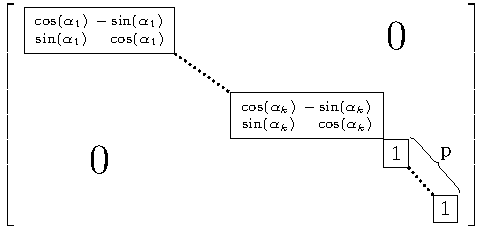
\includegraphics{pictures/isometrymatrix.pdf}
    \end{center}\pause
    Et pour $\vv{\phi} \in O^{-}(\ev{E})$, à la place du dernier $1$ il y a un $-1$ (donc $p>0$).
  \end{proposition}
\end{frame}

% ~~~~~~~~~~~~~~~~~~~~~~~~~~~~~~~~~~~~~~~
\subsection{Décomposition}
% ~~~~~~~~~~~~~~~~~~~~~~~~~~~~~~~~~~~~~~~
% -----------
\begin{frame}{Décomposition des isométries en réflexions}
  Toute symétrie orthogonale par rapport à un sous espace vectoriel est une isométrie\pause, directe si la codimension de cet espace est paire\pause, ou indirecte si la codimension est impaire.\pause
  \begin{definition}
    Une symétrie orthogonale par rapport à un hyperplan est appelée une \alert{réflexion}.\pause\\
    \myemph{(Une réflexion est une isométrie indirecte.)}
  \end{definition}\pause
  \begin{proposition}
    Soient $\ev{E}$ de dimension $\dim\ev{E}=n$, et $\vv{\phi} \in O(\ev{E})$.\pause\\
    Alors $\vv{\phi}$ est le produit de $k (\leq n)$ réflexions : $\vv{\phi} = \rho_{1}\circ\cdots\circ\rho_{k}$.\pause\\
    Si $k$ est pair $\vv{\phi} \in O^{+}(\ev{E})$, si $k$ est impair $\vv{\phi} \in O^{-}(\ev{E})$.
  \end{proposition}
\end{frame}


% =======================================
\section{Isométries affines}
% =======================================

% ~~~~~~~~~~~~~~~~~~~~~~~~~~~~~~~~~~~~~~~
\subsection{Définition}
% ~~~~~~~~~~~~~~~~~~~~~~~~~~~~~~~~~~~~~~~
% -----------
\begin{frame}{Définition d'une isométrie affine}
  \begin{defprop}
    On dit qu'une application affine $\phi \in\aff(\ens{E})$ est une \alert{isométrie} si une des conditions équivalentes est satisfaite:
    \begin{itemize}[<+(1)->]
      \item $\forall A,B \in \ens{E},\ d(\phi(A),\phi(B)) = d(A,B)$;
      \item $\vv{\phi} \in O(\ev{E})$.
    \end{itemize}
  \end{defprop}\pause
  On note \alert{$\iso(\ens{E})$} l'ensemble des isométries de $\ens{E}$.\pause\\
  Ainsi que \alert{$\iso^{\pm}(\ens{E})$} l'ensemble des isométries dont la partie linéaire est dans $O^{\pm}(\ev{E})$.
\end{frame}

% ~~~~~~~~~~~~~~~~~~~~~~~~~~~~~~~~~~~~~~~
\subsection{Propriétés}
% ~~~~~~~~~~~~~~~~~~~~~~~~~~~~~~~~~~~~~~~
% -----------
\begin{frame}{Premières propriétés des isométries}
  \begin{itemize}[<+(1)->]
    \item $\iso(\ens{E})$ est un sous-groupe de $\aut(\ens{E})$.
    \item $\iso^{+}(\ens{E})$ est un sous-groupe de $\iso(\ens{E})$.
    \item Les translations sont des isométries (directes).
    \item Une homothétie de rapport $\lambda$ multiplie les distances par $|\lambda|$\pause ,
      et donc n'est isométrie que si c'est l'identité ou une symétrie centrale.
    \item $\phi \in\aff(\ens{E})$ est dite \alert{symétrie (affine) orthogonale} \uncover<+(1)->{(resp. \alert{réflexion})} s'il existe $\Omega \in \ens{E}$ telle que $\phi$ est une symétrie (vectorielle) orthogonale \uncover<.(1)->{(resp. réflexion)} dans $\ens{E}_{\Omega}$. \pause Les symétries orthogonales sont des isométries.
    \item Toute translation est le produit de deux réflexions.
  \end{itemize}
\end{frame}

% ~~~~~~~~~~~~~~~~~~~~~~~~~~~~~~~~~~~~~~~
\subsection{Structure}
% ~~~~~~~~~~~~~~~~~~~~~~~~~~~~~~~~~~~~~~~
% -----------
\begin{frame}{Structure des isométries affines}
  \begin{lemma}
    Soit $\vv{\phi} \in O(\ev{E})$, alors $\ev{E} = \ker(\vv{\phi}-\id)\poplus\im(\vv{\phi}-\id)$.
  \end{lemma}\pause
  \begin{proposition}
    Soit $\phi \in\iso(\ens{E})$, alors
    \begin{itemize}[<+(1)->]
      \item soit $\phi$ possède un point fixe $\Omega$, et dans ce cas $\phi \in O(\ens{E}_{\Omega})$,
      \item soit il existe un unique $\vv{v} (\neq 0)$, vecteur fixe de $\vv{\phi}$, tel que $T_{\vv{v}}\circ\phi = \phi\circ T_{\vv{v}}$ possède \uncover<+(1)->{(au moins)} un point fixe.
    \end{itemize}
  \end{proposition}
\end{frame}

% ~~~~~~~~~~~~~~~~~~~~~~~~~~~~~~~~~~~~~~~
\subsection{Petites dimensions}
% ~~~~~~~~~~~~~~~~~~~~~~~~~~~~~~~~~~~~~~~
% -----------
\begin{frame}{Dimensions 1 et 2}
  \begin{itemize}[<+(1)->]
    \item $\phi \in \iso(\mathbb{R})$ $\Rightarrow$ $\phi(x) = \pm x +b$.\pause\\
    \myemph{($\phi$ est la composée d'au plus $2$ réflexions.)}
    \item $\iso(\mathbb{R}^{2}) = \iso^{+}(\mathbb{R}^{2}) \sqcup \iso^{-}(\mathbb{R}^{2})$.
      \begin{itemize}[<+(1)->]
        \item $\phi\in\iso^{+}(\mathbb{R}^{2})$ ssi\pause
          \begin{itemize}[<.(1)->]
            \item $\phi = R_{\Omega,\alpha}$ est la rotation de centre $\Omega$ d'angle $\alpha$\pause, ou
            \item $\phi = T_{\vv{v}}$ est une translation.
          \end{itemize}
        \item $\phi\in\iso^{-}(\mathbb{R}^{2})$ ssi\pause
          \begin{itemize}[<.(1)->]
            \item $\phi = S_{\ens{D}}$ est la symétrie par rapport à une droite affine $\ens{D}$\pause, ou
            \item $\phi = T_{\vv{v}}\circ S_{\ens{D}}$ avec $\vv{v}\neq0$ un vecteur fixe par la symétrie $\vv{\phi}$\pause\ (c.-à-d. $\vv{\phi} \in \ev{D}$)\pause, et dans ce cas on dit que $\phi$ est une \alert{symétrie glissée}.
          \end{itemize}
      \end{itemize}\pause
    \myemph{($\phi$ est la composée d'au plus $3$ réflexions.)}
  \end{itemize}
\end{frame}

% -----------
\begin{frame}{Les isométries affines de $\mathbb{C}$}
  \textit{Rappel :} Les applications affines de l'espace euclidien $\mathbb{C}$ sont de la forme $z \mapsto \alpha z+\beta\overline{z}+\gamma$.\pause\medskip

  $\iso(\mathbb{C}) = \iso^{+}(\mathbb{C}) \sqcup \iso^{-}(\mathbb{C})$
  \begin{itemize}[<+(1)->]
    \item $\phi \in \iso^{+}(\mathbb{C})$ ssi $\phi(z)=az+b$ avec $|a|=1$.
      \begin{itemize}[<+(1)->]
        \item Si $a \neq 1$, alors $\phi$ est la rotation de centre $\frac{b}{1-a}$.
        \item Si $a=1$, alors $\phi$ est la translation de $b$.
      \end{itemize}
    \item $\phi \in \iso^{-}(\mathbb{C})$ ssi $\phi(z)=a\overline{z}+b$ avec $|a|=1$.
      \begin{itemize}[<+(1)->]
        \item Si $\overline{a}b^{2} \in \mathbb{R}_{-}$, alors $\phi$ est une symétrie d'axe $\sqrt{a}\mathbb{R}+b/2$.
        \item Sinon $\phi$ est une symétrie glissée.
      \end{itemize}
  \end{itemize}
\end{frame}
% -----------
\begin{frame}{Dimension 3}
    $\iso(\mathbb{R}^{3}) = \iso^{+}(\mathbb{R}^{3}) \sqcup \iso^{-}(\mathbb{R}^{3})$.
      \begin{itemize}[<+(1)->]
        \item $\phi\in\iso^{+}(\mathbb{R}^{3})$ ssi
          \begin{itemize}[<+(1)->]
            \item $\phi = R_{\ens{D},\alpha}$ est la rotation d'angle $\alpha$ autour de l'axe $\ens{D}$, ou bien
            \item $\phi = T_{\vv{v}}\circ R_{\ens{D},\alpha}$, avec $\ev{D}=\affspan{\vv{v}}$
            \begin{itemize}[<+(1)->]
              \item si $\alpha=0$, c.-à-d. $\phi = T_{\vv{v}}$, c'est une translation,
              \item si $\alpha\neq 0$, on dit que $\phi$ est un \alert{vissage} d'axe $\ens{D}$ et d'angle $\alpha$.
            \end{itemize}
          \end{itemize}
        \item $\phi\in\iso^{-}(\mathbb{R}^{3})$ ssi
          \begin{itemize}[<+(1)->]
            \item $\phi = R_{\ens{D},\alpha}\circ S_{\ens{H}}$ avec $\ens{D}\perp\ens{H}$
            \begin{itemize}[<+(1)->]
              \item si $\alpha=0$, c.-à-d. $\phi = S_{\ens{H}}$, est la symétrie par rapport au plan affine $\ens{H}$
              \item si $\alpha\neq 0$, on dit que $\phi$ est une \alert{anti-rotation}.
            \end{itemize}
            \item $\phi = T_{\vv{v}}\circ S_{\ens{H}}$ avec $\vv{v}\neq0$ est un vecteur fixe par la symétrie $\vv{\phi}$\pause, et dans ce cas on dit que $\phi$ est une \alert{symétrie glissée}.
          \end{itemize}
      \end{itemize}\pause
    \myemph{($\phi$ est la composée d'au plus $4$ réflexions.)}
\end{frame}

% ~~~~~~~~~~~~~~~~~~~~~~~~~~~~~~~~~~~~~~~
\subsection{Décomposition}
% ~~~~~~~~~~~~~~~~~~~~~~~~~~~~~~~~~~~~~~~
% -----------
\begin{frame}{Décomposition des isométries en réflexions}
  \myemph{Rappel : Une réflexion est une isométrie indirecte.}\pause
  \begin{proposition}
    Soient $\ens{E}$ un espace affine de dimension $n$, et $\phi \in \iso(\ens{E})$.\pause\\
    Alors $\phi$ est le produit de $k (\leq n+1)$ réflexions :
    \[
      \phi = \rho_{1}\circ\cdots\circ\rho_{k}.
    \]\pause
    Si $k$ est pair $\phi \in \iso^{+}(\ens{E})$, et si $k$ est impair $\phi \in \iso^{-}(\ens{E})$.
  \end{proposition}
\end{frame}

% =======================================
\section{Similitudes}
% =======================================

% ~~~~~~~~~~~~~~~~~~~~~~~~~~~~~~~~~~~~~~~
\subsection{Définition}
% ~~~~~~~~~~~~~~~~~~~~~~~~~~~~~~~~~~~~~~~
% -----------
\begin{frame}{Définition d'une similitude}
  \begin{definition}
    \begin{itemize}[<+(1)->]
      \item Une application linéaire $\vv{\phi} \in \lin(\ev{E})$ est dite \alert{similitude vectorielle} si elle multiplie les normes par une constante $k > 0$ :
      \[
          \norm{\vv{\phi}(\vv{v})} = k\norm{\vv{v}},\qquad \forall \vv{v} \in \ev{E}.
      \]
      \item Une application affine $\phi  \in \aff(E)$ est dite \alert{similitude affine} si elle multiplie les distances par une constante $k > 0$ :
      \[
          d(\phi(A),\phi(B)) = k\!\cdot\!d(A,B),\qquad \forall A,B \in \ens{E}.
      \]
    \end{itemize}\pause
    Le nombre strictement positif $k$ est dit \alert{rapport de la similitude}.
  \end{definition}
\end{frame}

% ~~~~~~~~~~~~~~~~~~~~~~~~~~~~~~~~~~~~~~~
\subsection{Propriétés}
% ~~~~~~~~~~~~~~~~~~~~~~~~~~~~~~~~~~~~~~~
% -----------
\begin{frame}{Propriétés des similitudes}
  \begin{itemize}[<+(1)->]
    \item Une application affine est une similitude ssi sa partie linéaire est une similitude vectorielle.
    \item Les isométries sont des similitudes ($k=1$).
    \item Toute similitude vectorielle se décompose de façon unique en $\vv{\phi} = \vv{h}_{k}\circ \vv{\psi}$, où $\vv{h}_{k}$ est une homothétie de rapport $k > 0$ et $\vv{\psi}$ est une isométrie.
    \item Une similitude est dite \alert{directe} (resp. \alert{indirecte}) si son déterminant est positif (resp. négatif).
    \item Les similitudes sont des automorphismes (vectoriels, affines). L'inverse d'une similitude de rapport $k$ est une similitude de rapport $1/k$.
    \item Les similitudes vectorielles (resp. affines, resp. directes) forment un groupe.
  \end{itemize}
\end{frame}
% -----------
\begin{frame}{Propriétés des similitudes (bis)}
  \begin{itemize}[<+(1)->]
    \item Toute similitude affine, qui n'est pas une isométrie, possède un unique point fixe, dit \alert{le centre de la similitude}.
    \item Les similitudes préservent les angles.
    \item En particulier :
    \begin{itemize}[<+(1)->]
      \item Les similitudes préservent les sous-espaces parallèles.
      \item Les similitudes préservent les sous-espaces orthogonaux (perpendiculaires).
    \end{itemize}
    \item L'image d'une sphère par une similitude est une sphère.
  \end{itemize}
\end{frame}

\end{document}
